\documentclass[comsoc,final]{IEEEtran}
\usepackage[utf8]{inputenc}
\usepackage[T1]{fontenc}
\usepackage[zerostyle=b]{newtxtt}
\usepackage{subcaption}
\usepackage[inline]{enumitem}
\usepackage{booktabs}
\usepackage{multirow}

\usepackage[draft]{graphicx}
\graphicspath{{figs/}}
\IEEEoverridecommandlockouts

\usepackage{amsmath,amssymb,amsfonts}
\usepackage{algorithmic}
\usepackage{textcomp}
\usepackage{xcolor}
\usepackage{lipsum}
\usepackage[english]{babel}
\usepackage{csquotes}

\newcommand{\todo}[1]{\textcolor{red}{#1}}

\usepackage{hyperref}
\hypersetup{
    colorlinks=true,
    linkcolor=blue,
    filecolor=magenta,      
    urlcolor=teal,
    pdftitle={Iscc2023 Paper}
}
\usepackage{xurl}


\usepackage[style=ieee,backend=biber,doi=false,url=true,maxnames=3]{biblatex}
\AtEveryBibitem{%
  \clearfield{note}%
}
\addbibresource{tebaka2023.bib}

\begin{document}    % 6 Pagine, Double Column

\title{\textsc{TEBAKA}: Territorial Basic Knowledge Acquisition. An Agritech Project for Italy: Results on Self-Supervised Semantic Segmentation}
%\thanks{Tebaka thanks}
\author{\IEEEauthorblockN{Lorenzo Epifani, Antonio Caruso}\\
\IEEEauthorblockA{\textit{Dept. of Mathematics and Physics "Ennio de Giorgi", University of Salento, Lecce, Italy}}}

\maketitle

\begin{abstract}
Emerging technologies, such as Remote Sensing from Satellites and Drones, 
Internet of Things (IoT), Deep Learning, could be utilized to make informed decisions aimed to increase crop production. We provide an overview of \textsc{TEBAKA}, an Italian national project on \emph{Smart Farming} and discuss its relevance in the overall scenario of national or international project. We emphasize the originality of the project, and in particular the research on new advanced data-driven ML models that better integrate all knowledge from the domain.
We presented the task of \emph{image semantic segmentation} of olive trees or rows of grape plants and show an original Self-Supervised Deep Learning Network that produce the segmentation with high accuracy. Furthermore, we discuss the results and present some idea that would be part of the 
project activities for the next year.
\end{abstract}

\begin{IEEEkeywords}
digital agriculture, precision agriculture, satellite images, deep learning, machine learning,
sensor networks and iot
\end{IEEEkeywords}


\section{Introduction}
% general intro to agritech and relevance for computer science.

The enabling technologies of distributed sensor networks, internet of things, remote sensing using multi-spectral cameras on satellites, drones and aerial platforms, together with smart decision support systems are key contributors for the emerging field of \emph{Digital Agriculture} (DA) or \emph{Agriculture 4.0} \cite{de2018agriculture}. 
This is an \emph{umbrella term} used to designate the transformation of farming that includes digitalization and automation of farming tasks. This area of research encompass a new vision of the farming industry as a cyber-physical farm, and includes all technological areas such as: big-data platforms, machine learning and data-driven models to relate the observations of the phenological stages of plants with field yield and crop quality. 

The high-level goal is to support agronomist with \emph{Precision Agriculture} management practices, to better solve the challenges and demand of an increasing world-population, rising production costs (like energy), labor shortages, climate and environmental changes (like water resource scarcity). It leverages extensive knowledge acquisition using remote sensing technologies, and on-the-field deployment of sensors and IoT networks, to improve knowledge acquisition and situated situation awareness, to maximize resource usage and crop yield while minimizing associated costs.

In the United States, the use of yield-maps and soil maps are adopted only by 5 to 25 percent of total U.S. farms; on the other hand, automated guidance, has increased sharply, with the advance in deep-learning applied to computer vision, and it is applied to over 50 percent of the cultivated areas. A good survey of the trend in the technology evolution of a \emph{Smart Farm} in the USA is in \cite{mcfadden2023precision}. USDA (The U.S. Department of Agriculture) is investing up to $2.8$ billion in $70$ selected projects under the first Partnerships for Climate-Smart Commodities funding pool, as a part of the Inflation Reduction Act.


\begin{figure}
    \centering
    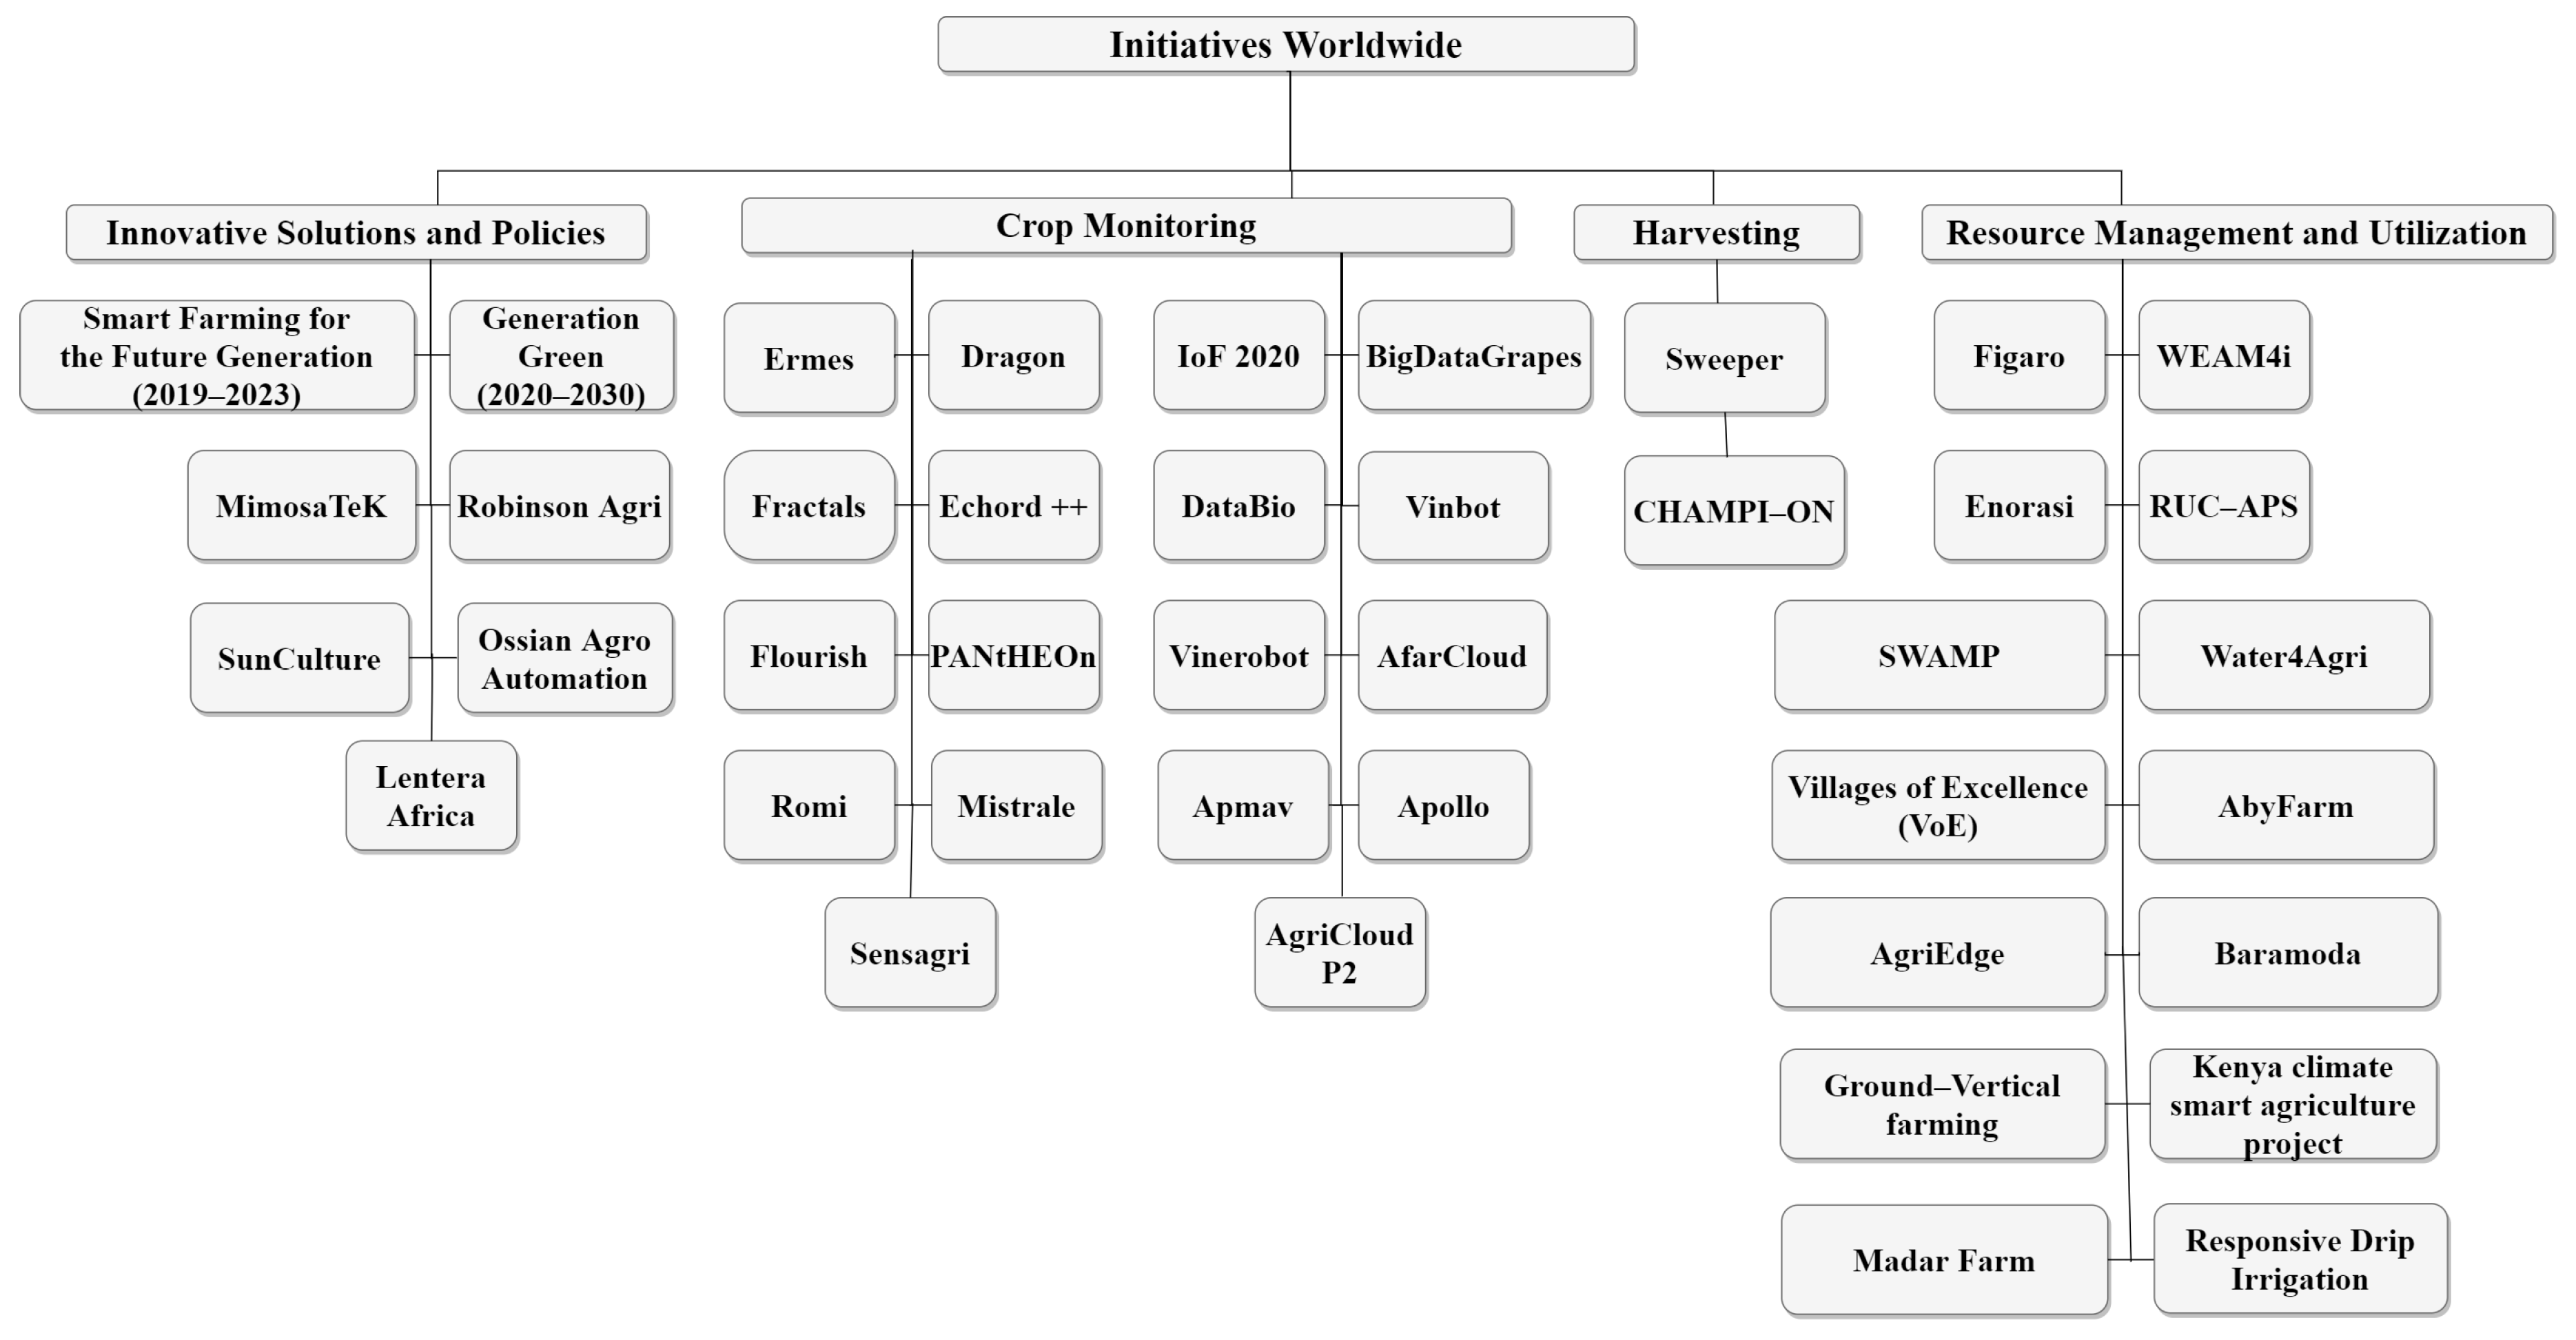
\includegraphics[width=\columnwidth]{agriengineering-04-00029-g005}
    \caption{A classification of active European Union funded projects in the area of Digital Agriculture (from \cite{agriengineering4020029})}
    \label{fig:euprojects}
\end{figure}

In Europe, the European Community has funded many projects that integrate ICT technologies and Digital Agriculture, we see in Figure \ref{fig:euprojects} from \cite{agriengineering4020029} a collection of active research project and startups, classified in different areas, such as:  \emph{Crop Monitoring}  (the largest one), \emph{Harvesting}, optimization of \emph{Resource Managements} and \emph{Innovative Policies and Solutions} with more than $41$ initiatives. In Table \ref{fig:table-worldwide} another list of worldwide projects that are actually funded, with a increasing role for African and Middle-East countries.

In this paper, we present the activities of \textsc{TEBAKA}: a national project funded by PON-FESN (European Union Social Fund) dedicated to develop the adoption of Digital Agriculture in the south part of Italy (Mezzogiorno) and in particular in Apulia (Puglia). The project span four years, from 2020 to 2024 and with an overall budget of 8.5 Million Euro it put together more than 20 partners from industry, two university, several national research institutions of Italian CNR, and private partners with a mixed background (someone more oriented to ICT services, someone more related to agronomy). 
We discuss the project in the following section, but we want to summarize here the key ideas involved. The project goals are a new generation of decision support systems, for agronomists, for the culture of grain, vine and olive. For this goal, the project comprise a large campaign of data acquisition, with measurements taken directly on the culture and soil, spanning two full year. Moreover, all measurements will be taken at the same time of satellite observation (with Sentinel 2), drone observations equipped with a multi-spectral camera and with aircraft. These four levels of observation are unique in all the projects presented in the previous discussion, they allow a \emph{pyramidal representation} at different spatial resolution of the phenomena observed, and in different time. On top of this raw observations, we develop data-driven models (mostly based on \emph{neural networks}) that extract features from images related with the specific conditions of the annual crop life cycle.

The rest of the paper is organized as follows: in \ref{sec:tebaka} we review the project structure and management organization, the partnership and roles, the research goals and actual status; in \ref{sec:activities} we present some interesting original results. An important task in the overall pipeline of analysis is a proper \emph{semantic segmentation} of the plant crown (foliage), i.e a mask that label each pixel of an image taken from UAV, as 'terrain' or 'green area'; we present an original self-supervised approach to the problem and discuss the results, in \ref{sec:related} we collected some of the most relevant works that shape the area, and finally we have drawn in \ref{sec:conclusion} the conclusions.

\begin{figure}
    \centering
    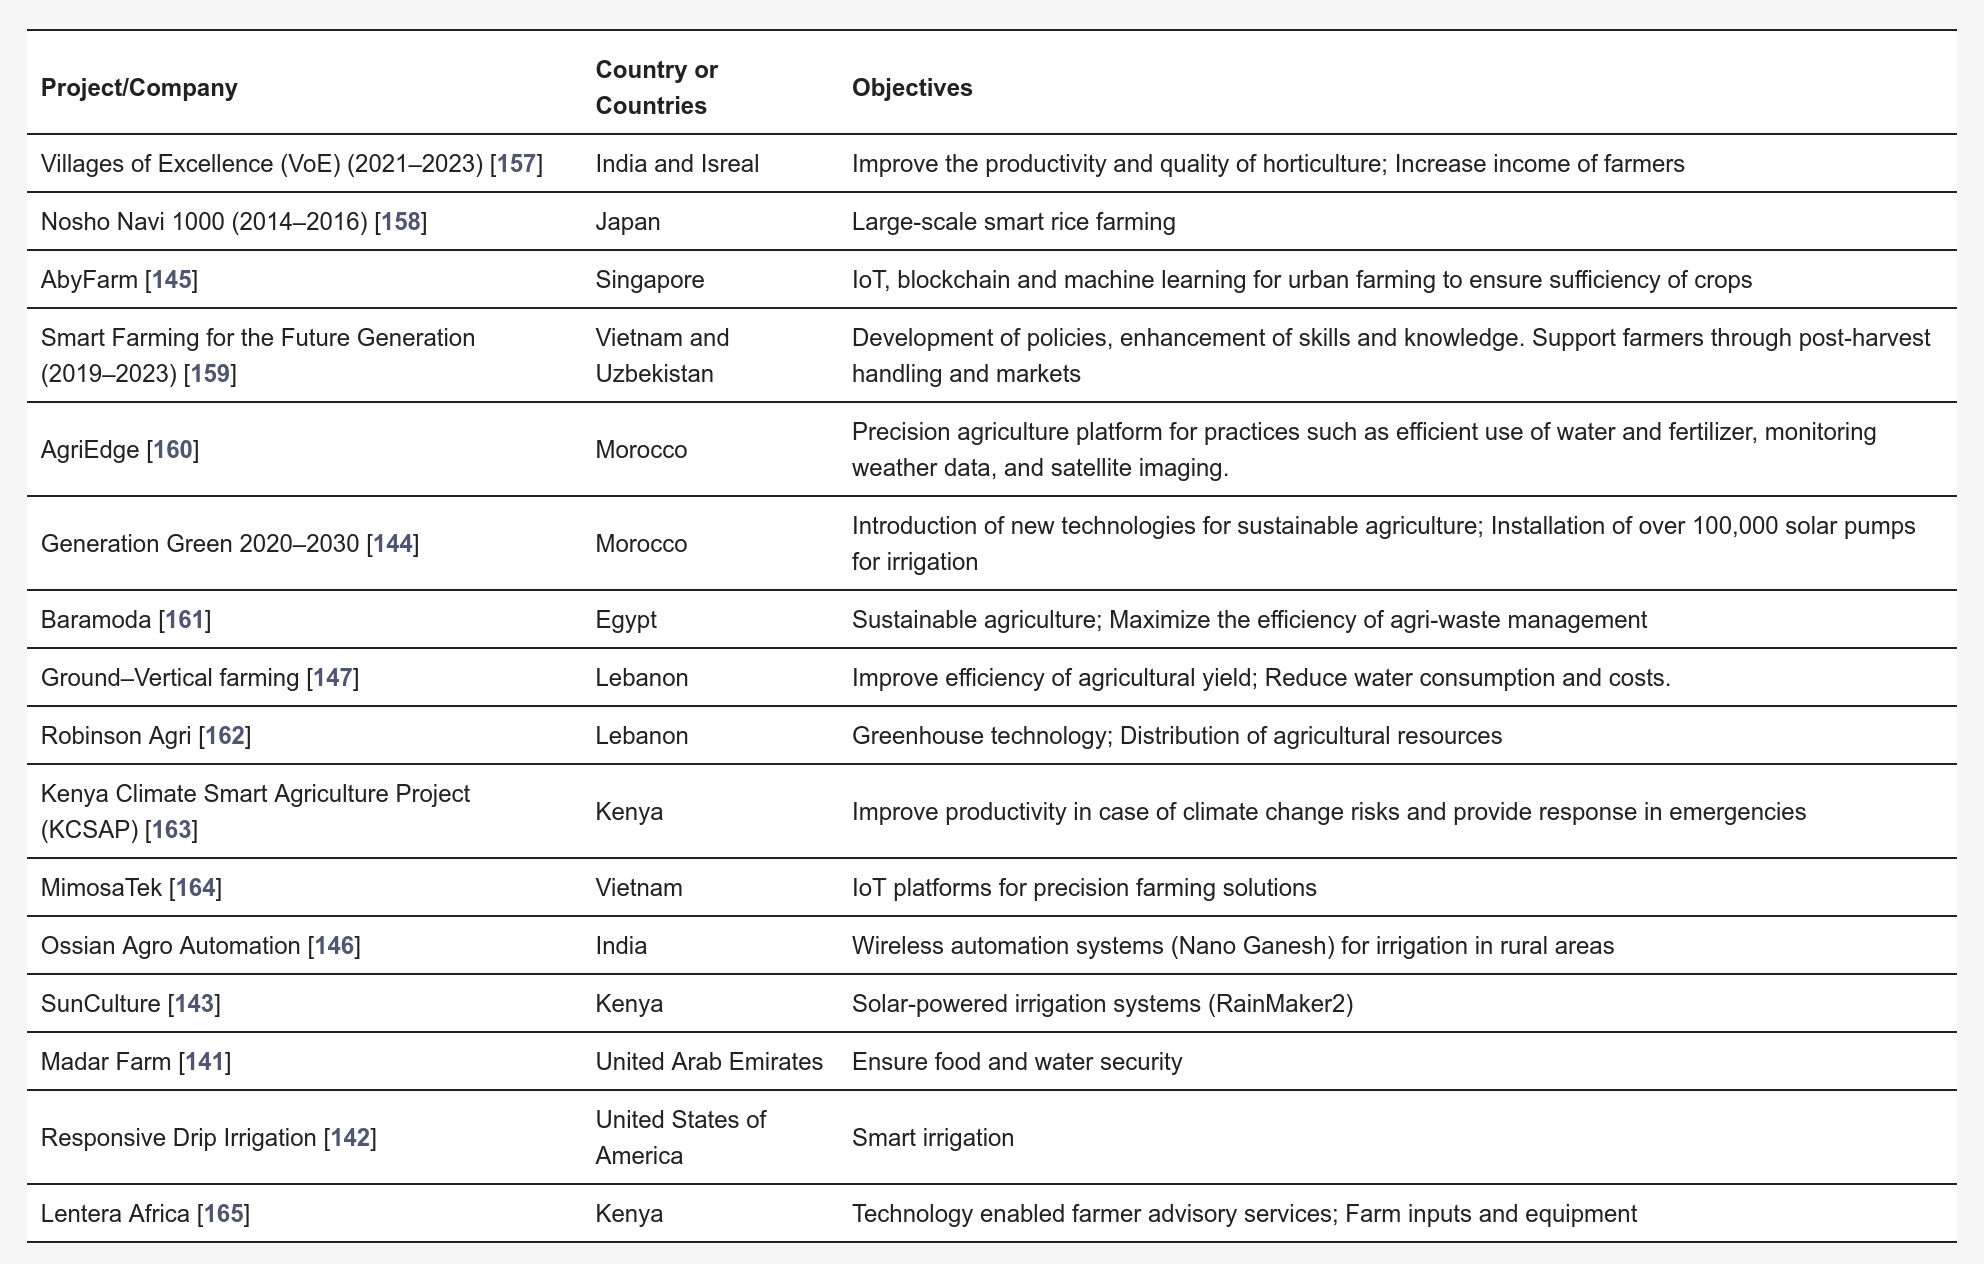
\includegraphics[width=\columnwidth]{research-table}
    \caption{A list of worldwide projects related to the area of Digital Agriculture (from \cite{agriengineering4020029})}
    \label{fig:table-worldwide}
\end{figure}

%--------- end of intro

\section{Tebaka Project Description}\label{sec:tebaka}

Tebaka is a “\emph{platform}” solution for crops of grain, vines and olive, all of which are significantly present in the sud of Italy, and will operate through stages of knowledge development and design / realization of prototype solutions that is articulated in four years (2020/2024) with the four major phases described in the following.

\textsc{Data Acquisition:}

\begin{itemize}
\item Analysis of the territory of Puglia, identification of the areas and parcels cultivated to observe, definition / authorization of the operational missions and their verification.
\item Definition of payload and cargo platforms of sensors to be used (on already operational satellites and on aircraft and land systems to integrate / develop), development of a control room for mission management and operational integration with a data acquisition and processing center.
\item Definition of data acquisition criteria from various platforms / pay loads during the various missions envisaged, verification of operational adequacy in the identified territories and basic processing of acquired data through representation in thematic maps.
\end{itemize}

\textsc{Analysis and Modelling Phase:}

\begin{itemize}
\item Definition of the theoretical models of the annual production cycles of the agricultural crops considered, of the fusion criteria of data from multisensory sources, of the criteria for the analysis of the data acquired in the missions, of the criteria for the realization of the data driven models with the use of artificial intelligence logic and deep learning, of criteria for their integration with theoretical models, and the implementation of integrated and validated basic models.
\item Development of Intensive Data Acquisition Activity from Payloads / Platforms for refinement of models, realized by means of large amounts of data processing, definition of criteria for identifying potential critical factors and development of models / support decision systems for their management, development of the design and the prototype of the complete system.
\end{itemize}

\textsc{Prototype Development:}

\begin{itemize}
\item Realization of the prototype of an integrated platform composed of technological systems (satellites, manned and unmanned aircraft, manned and unmanned land vehicles and fixed stations, payloads of sensors with different characteristics and performance, storage environments of large amounts of data and applications in the field of artificial intelligence for data manipulation;
\item The building of data driven models; the development of models and relationships between the observed phenomena elements realized with machine learning logic, data analysis, decision support systems) in order to develop a product / service for the world of crops with different types of extension on the territory (horizontal for grain, vertical for vine and mixed for the olive tree, others with comparable characteristics) to be offered to various actors operating in the world of innovative agriculture such as Public Organizations, Category Associations, Service Providers, Agricultural Companies, possibly complementing the proposed solution with other complementary existing or developing ones.
\end{itemize}

The proposed project has as its ultimate goal the creation of an innovative product for agriculture, in particular to provide guidance in the initial stages of grows, and to guide the best-performing actions. 
During the development of the project, a comparison will be made between the participants and external stakeholders to evaluate the opportunity to realize a spin-off that, through the acquisition of the platform as a basis for providing services on the market.


%% ------------------------------- ciccia ---------------

\section{Self-Supervised Semantic Segmentation of Plant Crown}\label{sec:activities}
% Image analysis using deep learning, role, goals result.

Segmentation is a recurrent task in literature regarding precision agriculture: the information provided by a pixel-wise classification map can by used to solve different domain specific tasks (\cite{s21051617,rs14061523,Egli20201}), e.g. biovolume estimation, tree crowns mapping, estimate the distribution of the population for different species , monitoring changes in green areas. 
%\todo{list someone}
We introduce this task, in TEBAKA, in order to monitor the grow of
plants and in particular the \emph{volumetric leaf area} and its evolution across time.

The two main remote sensing technologies that have been used over the years are satellite and UAV imagery, each one having his pros and cons. Even if satellite imagery has also been used successfully by several authors\cite{ruswurm_multi-temporal_2018,daudt_fully_2018,ienco_land_2017},
the unmanned aerial vehicles (UAVs) have proven to be a game-changing technology for various reasons. The main one is that for the majority of agriculture challenges, there are strict resolution requirements that satellite imagery cannot satisfy. These requirements can be meet by UAV imagery while keeping costs acceptable. Satellite imagery is the best choice only if we have to deal with large scale observable phenomena\cite{gurumurthy_mango_2019,guirado_mask_2021}, since specific patterns can be observed only from a certain scale onward. For these reasons, we decided to choose UAV imagery as data source.

In agronomic, there are many well known indexes that are used to assign a score to each pixel. These indexes are often linear (or non-linear) combination of spectral channels, and have proven to be highly correlated to specific characteristics available in areas that have and index score above a certain threshold. The Normalized Difference Vegetation Index (NDVI) is an index, whose formula is:
    \[
    NDVI = \frac{NIR-R}{NIR+R}
    \]
    %\todo{L: aggiungere descrizione NIR e motivo formula NDVI}
    %\todo{explain NIR, they don't know about it, and the general idea of why ndvi is computed in that way..find everything on wikipedia, just one more phrase}
    The choice of these two light bands is based on the fact that plants absorb light energy in the red band for chlorophyll photosynthesis and instead reflect a lot of energy in the near-infrared band due to the cell structure of the plants themselves. Therefore, the NDVI exploits these properties to measure the amount of chlorophyll and foliage density present in vegetation.
The index ranges from a value of -1 to +1, where a value of -1 indicates the presence of water or snow, 0 indicates an unvegetated surface such as rocks or bare soil, and a value of +1 indicates extremely dense vegetation. In general, higher NDVI values correspond to higher vegetation density and plant health.
%The Normalized Difference Water Index (NDWI) is another index used to estimate the leaf water content at canopy level.
Even if NDVI thresholding can be used to produce a segmentation map of a UAV image, there are many issues that make it a non-optimal choice. Different objects with the same spectrum obtains the same score, even if they belong to different classes. Moreover, NDVI does not consider local properties and patterns. Image analysis through deep learning has proven to provide state-of-the-art solutions for instance/semantic segmentation in different domains. For this reason, this method has been widely used in precision agriculture in the last decade.

However, supervised deep learning methods require large, hand-labelled datasets, that are carefully prepared by domain experts, in fact, in all the works examined, and reviewed in the next section, the labelling is carried out by agronomists. In our work, we propose an original solution for the automatic labeling of UAV images containing vineyards and olive trees. We tested this method, by using this data-set to train a well-known semantic-segmentation neural network model, the entire system can be considered a self-supervised model, with the advantage that the self-labelling pipeline, can be used to label any plant species without the costly manual labor of a domain expert (in this case an agronomist). To the best of our knowledge, there is no other work using a similar solution in this domain, in particular we are not aware of a single method that can be used on more than a single culture type. 

The self supervised pipeline is a system that takes as input a hyper-spectral orthomosaic and returns the set $\mathcal{D}$: \[
\mathcal{D} = \{\, (x_i,y_i):i \in \{1...N\}\,\}
\] where $x_i$ represents the $i$-th tile of the input orthomosaic, $y_i$ is the ground truth mask for $x_i$ and $N$ is the total number of collected tiles i.e. the size of the dataset.
% \todo{explain what is $i$, i.e. the size of the dataset, introduce a variable (maybe, 'we consider N the size of the dataset and $i$ range over N}. OK
Masks and tiles have the same spatial resolution, but masks have only one channel, i.e. they are bitmaps, with the value of each pixel be equal to 0 (background) or 255 (vegetation) (we still use 8 bit for each pixel). This representation is useful for visualization purposes. During the development of the machine learning model, we represented 0 and 255 with the one-hot-encoding.
%\todo{it is a detail, or it is important?}

Only two classes have been assigned to speed up prototyping, but their number can be easily extended, i.e. by labelling each species with a different value. The self supervised pipeline (Figure \ref{fig:entirepipeline}) works as follow:

\begin{itemize}
    \item The NDVI is computed pixel-wise from the multispectral input orthomosaic and stored as a single-channel image. 
    $NIR$ (Near Infra Red) and $R$ (Red) bands are respectively stored in the 6th and the 10th channels of our source orthomosaic.
    \item The NDVI map is the input to a Tunable Denoising Module that is part of the self-supervised model. This component (shown in Figure \ref{fig:tunable_module}) is a stack of different well known image processing techniques executed sequentially. 
    The module is executed by fixing a set of parameters that govern its operation. In our experiments, the values of these parameters were found by drawing inspiration from the search criteria for hyperparameters used in machine learning (e.g. grid search inside intervals considered reasonable).
    This module produces the pixel-wise ground truth map for the entire hyperspectral source orthomosaic. The tunable parameters of this module are 5 (highlighted in red in previous image). Values $th_1$ and $th_2$ governs the two tresholding stages, while $sw$, $tw$ and $str$ respectively represents the search window size, the template window size and the strength of the fast non-local means denoising method. For the dilation and the erosion, we used kernels containing only 1 with size $3\times3$ and $5\times5$.
    An erosion follower by a dilation is called opening. The opening is a smoothing filter and the specific behavior depends on the kernel size and content. An opening preserve as much as possible regions having similar structure respect to the kernel, while removing those different. Our kernels with all 1's allow to remove isolated groups of pixels, while their dimension governs the minimum size that groups of pixels must have in order to be preserved. Kernel size and content could be governed introducing some parameters, although in our experiments we achieved good results with static kernels.
In our case, they serve to remove groups of isolated pixels classified as plants 
    %\todo{maybe write a single phrase on the high level task of this? like 'removing debris or small components in the image??}
    \item The orthomosaic/ground truth are both split in many tiles of a fixed size. We pairwise store each input tile and its corresponding ground truth tile. The size of the tiles was chosen consistently with the size of the input expected from the semantic segmentation deep learning model we trained.
\end{itemize}

Before storage, pairs of tiles containing insufficient information are discarded. Specifically, if the pixels in the truth map describing vegetation are fewer than a given threshold, then the pair is discarded. In our experiments, we labeled $906$ tiles (net of rejected ones) starting from $5$ UAV orthomosaics acquired in $2$ different areas of interest 
%\todo{and spanning an area of ..km$^2$}.
\begin{table}[htbp]
  \centering
  \caption{Area of interest}
  \label{tab:aoi}
  \begin{tabular}{c*{3}{c}}
\toprule
           & GSD     & Area (km$^2$)             & \# Flights  \\
    \midrule
    Area-0  & $10$cm/px& 0.072 & $3$  \\
    \cmidrule(l{0.5em}r{0.5em}){1-4}
    Area-1 & $3$cm/px & 0.005 & $ 2 $  \\
    \bottomrule
  \end{tabular}
\end{table}
Flights for the acquisition were performed in a temporal window spacing from the $26$ May $2022$ to $30$ Sep $2022$. The semantic segmentation model we chose for training is the U-Net 
\cite{ronneberger_u-net_2015}, with some modifications, 
%\todo{it is not up to you to write 'trivial' for tour job, you are selling something..so nothing is trivial}
for example making it capable of handling the 10 channels for the images in input. 
Tiles have a resolution of $572\times572$ pixel. The U-Net is able to classify the inner square having size $388\times388$ because it needs to evaluate the context around each pixel, leaving the pixels on the edge unclassified. However, it is possible to classify the entire orthomosaic by properly managing a sliding window and applying mirroring to the border tiles of the orthomosaic. The patches represent areas of 327 m$^2$  and $98$ m$^2$ for their respective areas of interest, according to spatial resolution of the orthomosaics from which they are sampled.


%In addition, we used a matrix full of 1's as the loss regularisation matrix, thus making it irrelevant. 

We chose U-Net over other similar architectures for several reasons: it has fewer parameters than competing networks. Moreover, it was originally proposed to solve a task of similar complexity (biomedical image segmentation) with excellent results, which were then replicated on use cases very similar to ours. Lastly, in these publications (and also in the original work) the U-Net was trained from scratch with datasets of comparable size to ours (often even smaller).
%\todo{if you don't need to reference the (a)(b)(c), why don't just write the paragraphs, without them??}

We performed several training runs in order to cross validate different hyperparameters: decay rate, learning rate, number of epochs, and batch size. 
In table \ref{tab:hyperpar} there are the hyperparameters of 3 models chosen from all those tested in cross-validation are shown, and in Figure \ref{fig:unet_models} we show how these models behave in inference.
%\todo{ok, and we are happy ;), so ....discuss the result of the training in fig 5.}
\begin{table}[htbp]
  \centering
  \caption{Hyperparameters settings \label{tab:hyperpar}}

  \begin{tabular}{c*{5}{c}}
    \toprule
    & \multirow{2}{*}{\shortstack{Learning\\rate}} & \multirow{2}{*}{\shortstack{Decay\\rate}}  & \multirow{2}{*}{\shortstack{Decay\\ each}} & \multirow{2}{*}{\shortstack{Epochs}} & \multirow{2}{*}{\shortstack{Batch\\size}} \\\\
    \midrule
    Model-0  & $5\cdot10^{-4}$ & $0.75$ & $40$ & $4$ & $5$ \\
    \cmidrule(l{0.5em}r{0.5em}){1-6}
    Model-1 & $5\cdot10^{-4}$ & $0.75$ & $40$ & 2 & 10 \\
    \cmidrule(l{0.5em}r{0.5em}){1-6}
    Model-2 & $5\cdot10^{-4}$ & $0.95$ & $20$ & 25 & 10 \\
    \bottomrule
  \end{tabular}
\end{table}
We choose not to use performance evaluation metrics commonly used in the literature for segmentation task (e.g. Intersection Over Union).
Our self-supervised labelling system represents an approximation of the labelling process that relies on domain experts, thus it tends to automatically label shadows as vegetation (this happens mainly in vineyard, Figure \ref{fig:input_gt}). Despite this, some of our trained U-Net models are unaffected by this issue (especially model-1) and can distinguish crowns from shadows. I can be observed that although model-1 is visually better than model-2 (Figure \ref{fig:unet_models}), a comparison with any metric would lead us astray as error is also present in the ground truth masks.
In our experiments, some models are able to generalize well because not all shadows are labelled as vegetation (especially in olive trees, but this also happens in many portions of vineyard). Models that are trained for too many epochs tend to overfit and label shadows as vegetation. This is especially evident in the case of vineyard.
This problem can be handled when generating the dataset by introducing asymmetrical opening kernels, in order to perform stronger erosion in the direction in which the shadow is present and/or weakening dilation in the same direction. This would add parameters to the self-supervised pipeline, increasing its complexity and the time required for fine-tuning. In the last section we discuss of possible future works to improve the model.

\begin{figure}
    \centering
    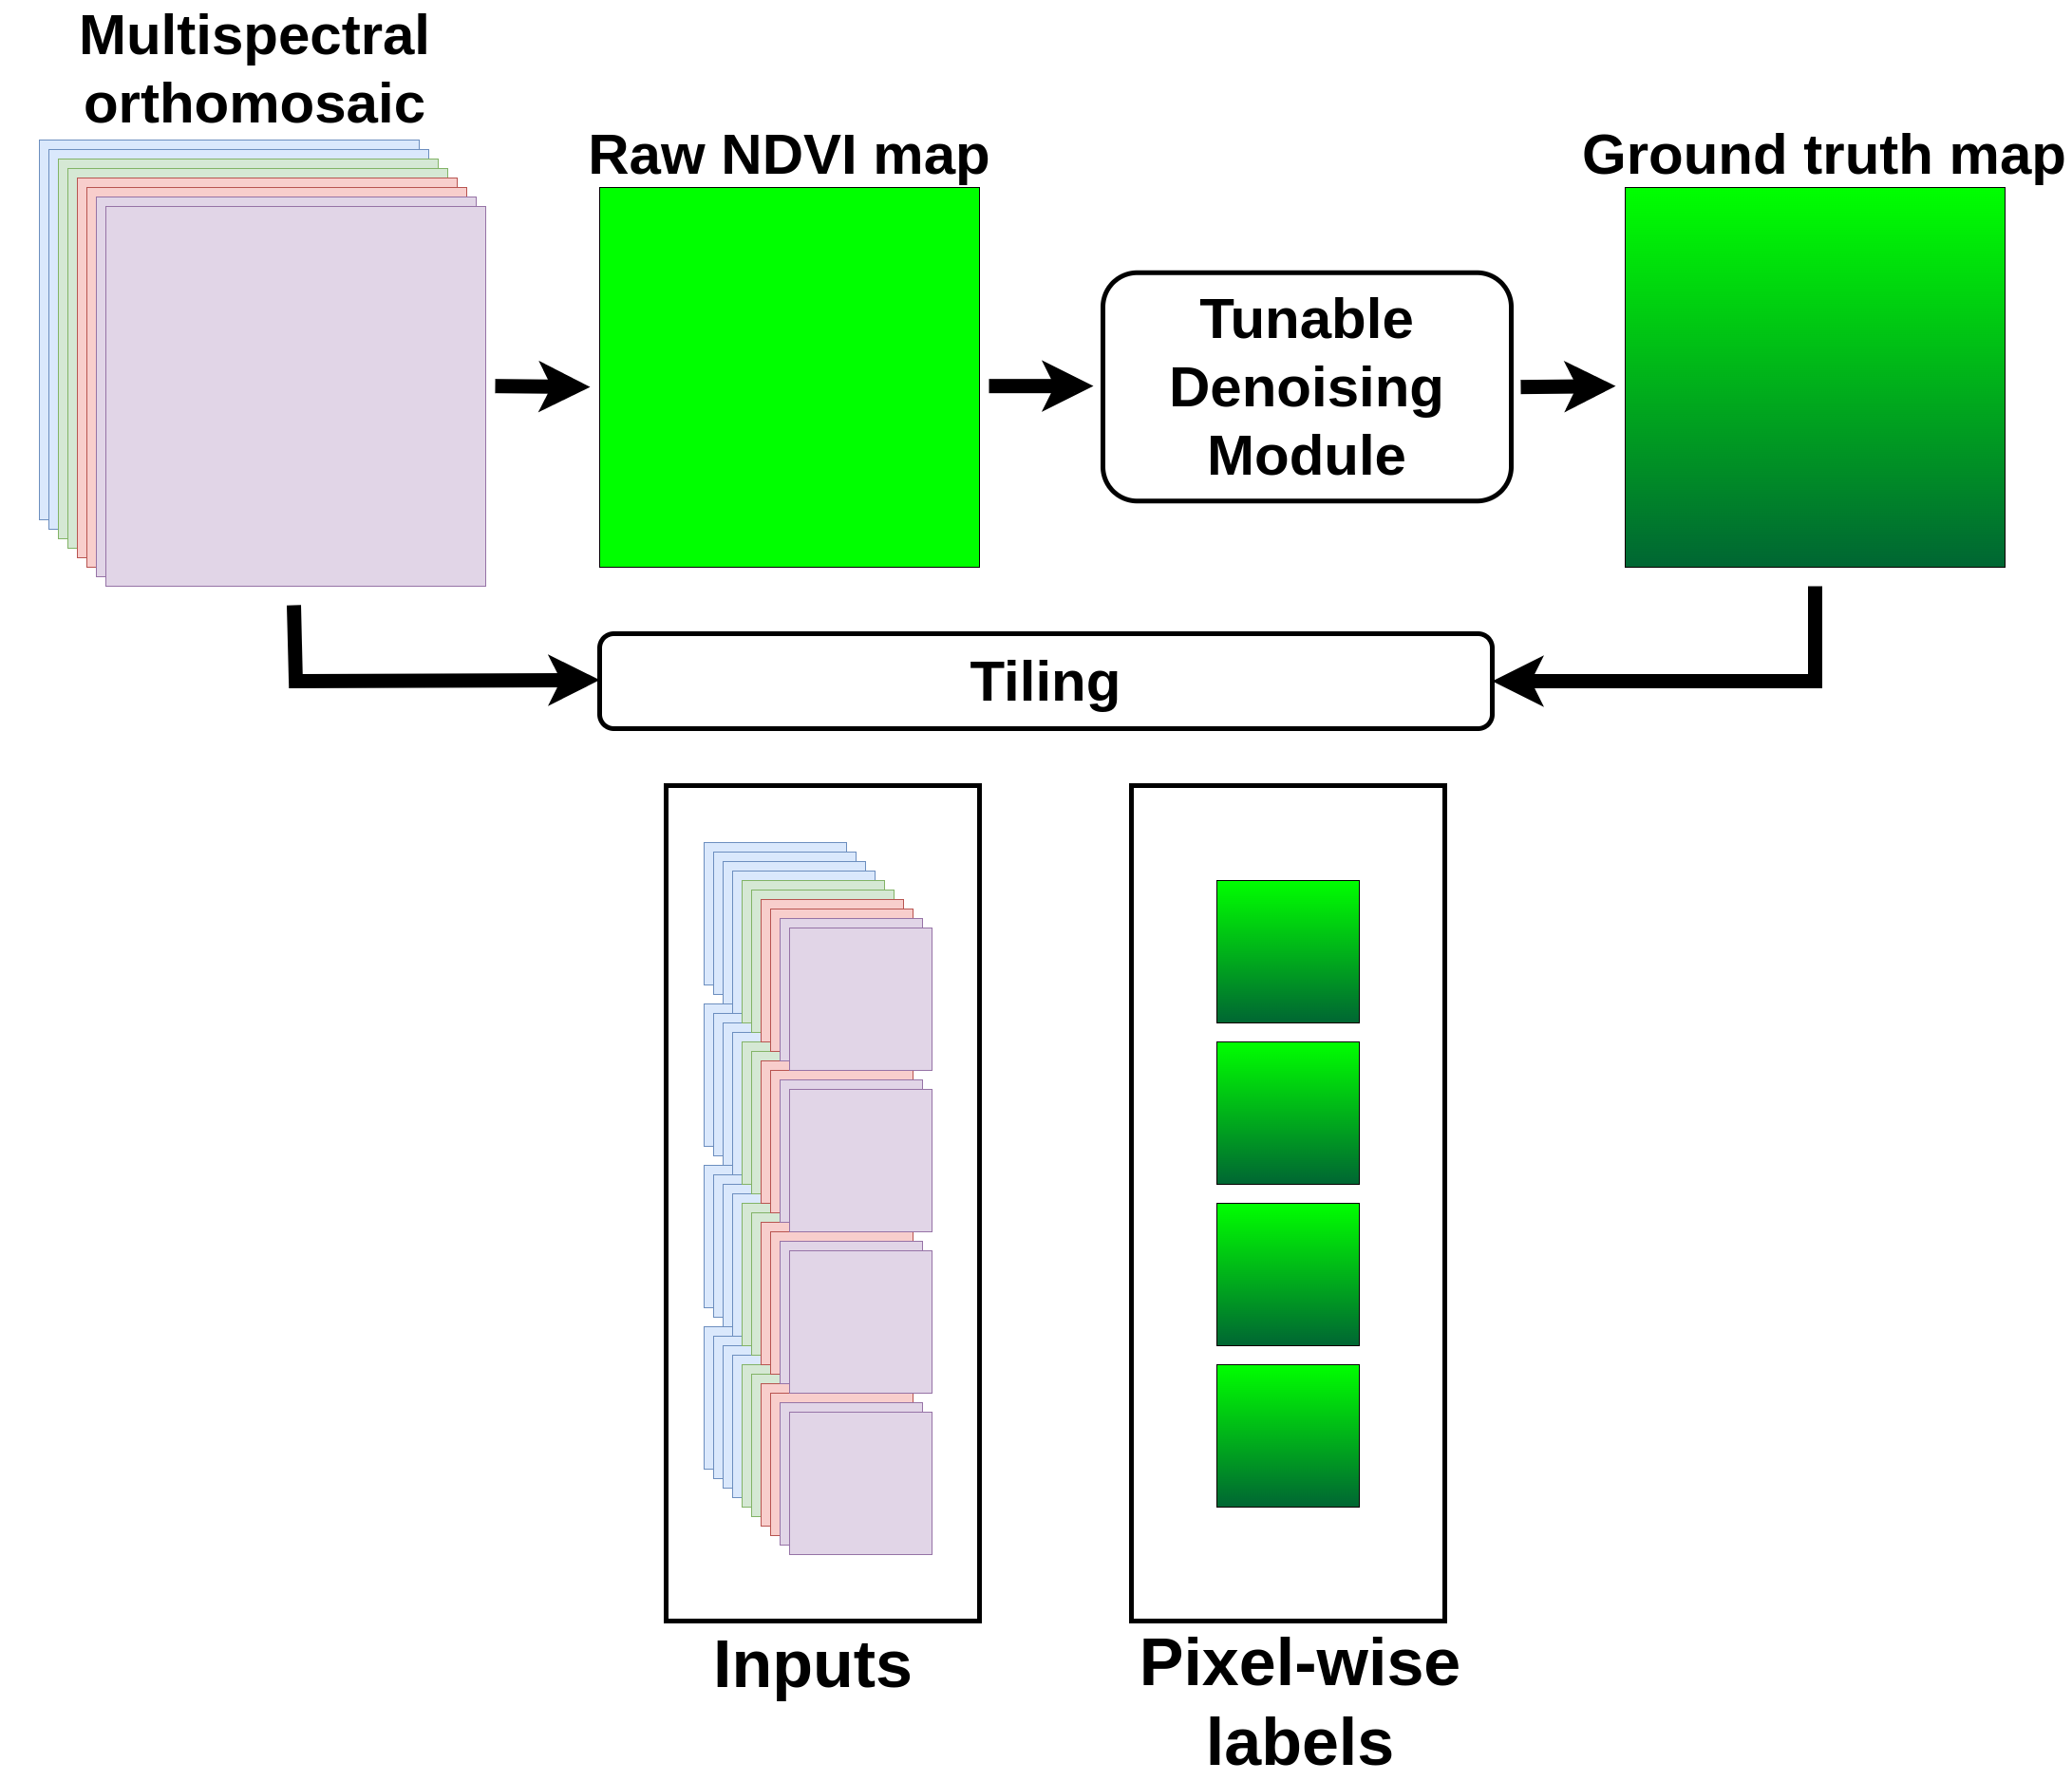
\includegraphics[width=0.8\columnwidth]{pipeline1}
    \caption{Graphical representation of the entire self-supervised pipeline.}
    \label{fig:entirepipeline}
\end{figure}

\begin{figure}
    \centering
    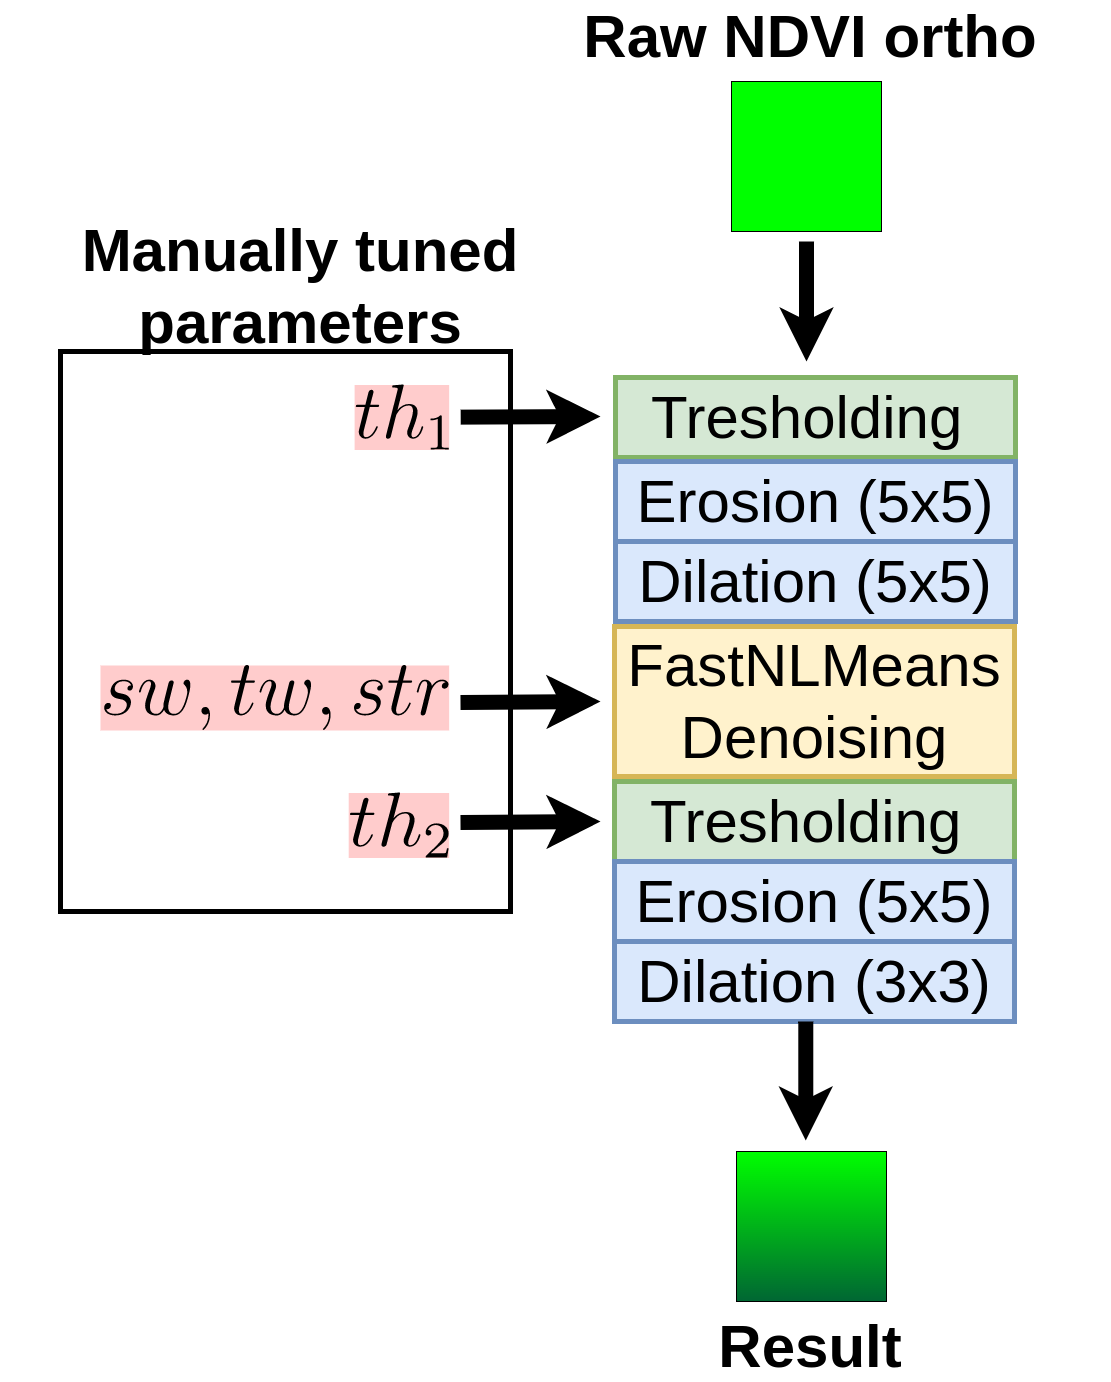
\includegraphics[width=0.75\columnwidth]{tunable_module}
    \caption{Schema of the Tunable Denoising Module.}
    \label{fig:tunable_module}
\end{figure}

\begin{figure}{\centering%
%
      \begin{subfigure}[b]{0.45\columnwidth}
         \centering
         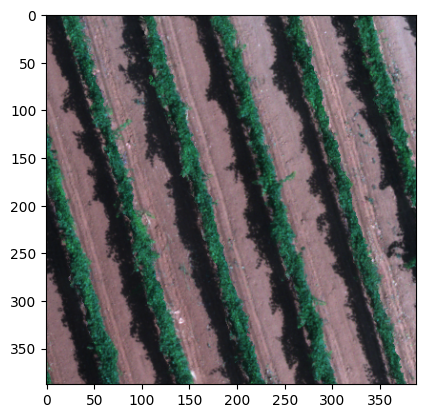
\includegraphics[width=\columnwidth]{vite}
         \caption{}
         \label{maskplot:a}
     \end{subfigure}%
%
     \begin{subfigure}[b]{0.45\columnwidth}
         \centering
         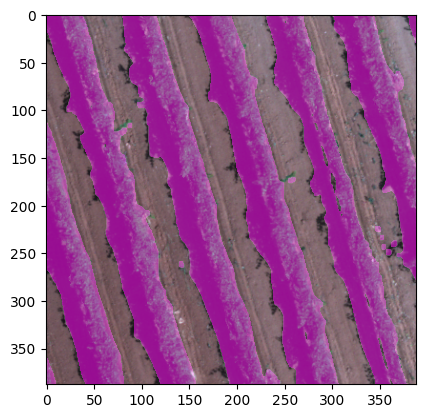
\includegraphics[width=\columnwidth]{vite_GT}
         \caption{}
         \label{maskplot:b}
     \end{subfigure}}\hfill
%       
     \begin{subfigure}[b]{0.45\columnwidth}
         \centering
         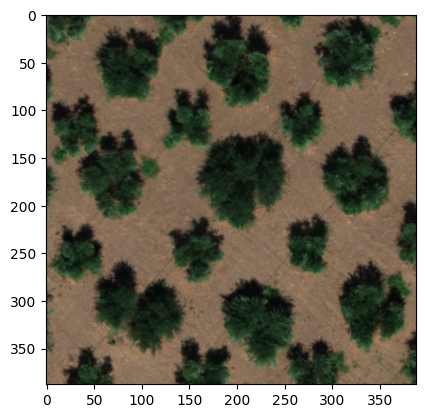
\includegraphics[width=\columnwidth]{ulivo}
         \caption{}
         \label{maskplot:c}
     \end{subfigure}%
%
     \begin{subfigure}[b]{0.45\columnwidth}
         \centering
         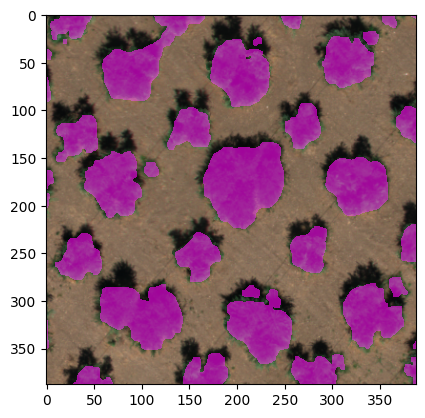
\includegraphics[width=\columnwidth]{ulivo_GT}
         \caption{}
         \label{maskplot:d}
     \end{subfigure}%
%        
     \caption{(a) Inner square of an input tile, vineyard; (b) Overlay between the previous input tile and the result produced by our self supervised pipeline; 
     %(c) Overlay between the vineyard input tile and his ground truth mask. 
     (c), (d) are the same but for olive trees.}
     % don't break lines manually NEVER
     \label{fig:input_gt}%
\end{figure}

\begin{figure}{\centering%
      \begin{subfigure}[b]{0.45\columnwidth}
         \centering 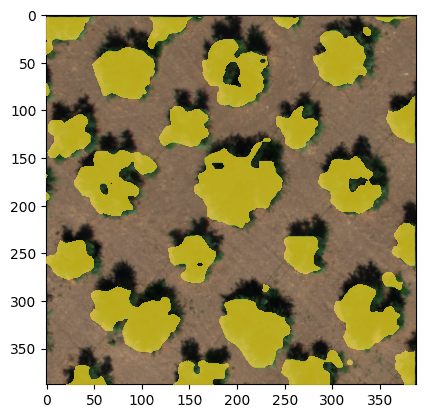
\includegraphics[width=\columnwidth]{ULIVO0INF}
     \end{subfigure}%
%
      \begin{subfigure}[b]{0.45\columnwidth}
         \centering 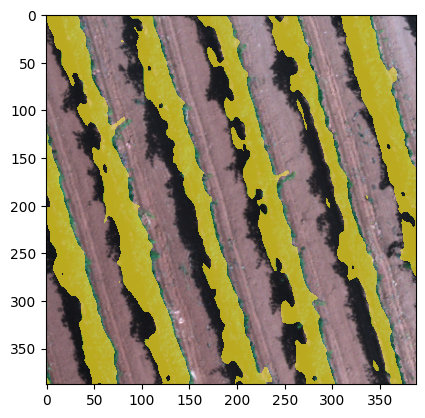
\includegraphics[width=\columnwidth]{VITE0INF}
     \end{subfigure}}
%       
      \begin{subfigure}[b]{0.45\columnwidth}
         \centering 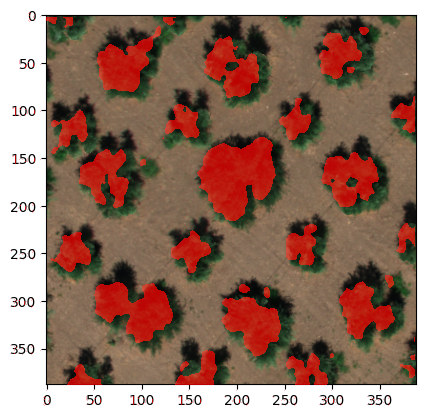
\includegraphics[width=\columnwidth]{ULIVO1INF}
     \end{subfigure}%
% 
      \begin{subfigure}[b]{0.45\columnwidth}
         \centering 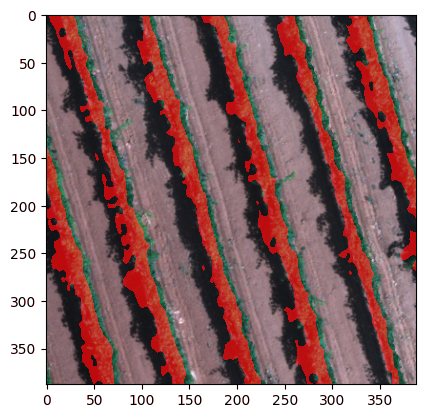
\includegraphics[width=\columnwidth]{VITE1INF}
     \end{subfigure}
%
      \begin{subfigure}[b]{0.45\columnwidth}
         \centering 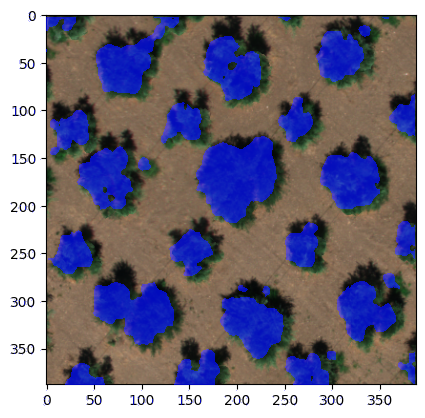
\includegraphics[width=\columnwidth]{ULIVO2INF}
     \end{subfigure}%
%       
      \begin{subfigure}[b]{0.45\columnwidth}
         \centering 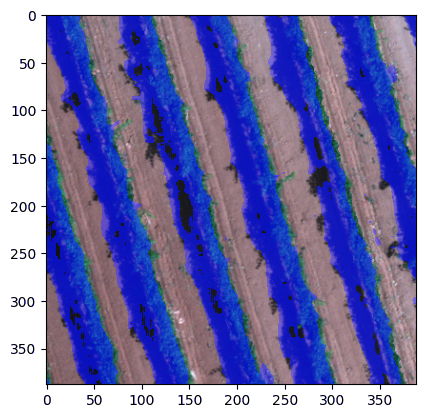
\includegraphics[width=\columnwidth]{VITE2INF}
     \end{subfigure}%
     \caption{Overlay between the input tiles and the result produced by our models. 
     Yellow is for model-0, red for model-1 and blue for model-2}\label{fig:unet_models}
\end{figure}

\section{Related Works}\label{sec:related}
% a panoramic view of the best literature, focus on technology.

Although the papers are quite heterogeneous it is possible to pool some features
on the method used by almost all authors. Each author is interested
in monitoring different areas with its own local characteristics and species, and therefore everyone
provides for themselves in the construction of the dataset. In general, almost all authors perform the acquisition UAV flights, orthomosaic tiling and the full dataset labeling performed by domain experts.
No work reviewed uses techniques for automatic or self-automatic labelling.
Safonova et al in \cite{s21051617} proposed a Mask R-CNN implementation to solve an instance segmentation task.
In this work, they used the Mask R-CNN model to identify (with 2 different classes) shadows and crowns of several olive trees featured in an orthomosaic.
The shadow was used to estimate the height of each tree. 
Ye et. al. in \cite{rs14061523} proposed an implementation of a stacked U-Net (also called U$^2$-Net) to solve a binary semantic segmentation task. 
The goal was to separate olive crown surface from the background. 
The nested structure of the chosen architecture has shown a great potential in capturing multiscale feature information.
Gurumurthy et al in \cite{gurumurthy_mango_2019} proposed a fully convolutional neural network for the instance segmentation of mango trees. 
This work aims to the individual crown detection in the target crop. 
Their approach is different: the selected model is first trained for the semantic segmentation of tree crowns. 
At this stage, the network produces a single map of scalars, each value of the map represents a score describing the probability that the observed pixel belongs to a canopy. 
In the next stage, the network is retrained by replacing the head so that it produces a map with the scores of 3 different classes. 
In this case, the classes represent the canopy, the background, and the intersection surface between the canopies. 
The two training steps use a differently labeled dataset.
Natesan et al. in \cite{Natesan2019475} proposed a Resnet 50-based CNN to classify patches containing tree crowns into 3 different classes (red pine, white pine, non-pine). 
Patches were extracted from an orthomosaic using a processing pipeline based on classical computer vision techniques. Gaussian Smoothing was first used on the DSM (digital surface model) followed by the marker controlled watershed segmentation algorithm (as in \cite{Vepakomma2018}). Thus, the ground truth of each extracted pach has been provided by a forestry expert. Egli et al in \cite{Egli20201} proposed a multiclass 4-layer lightweight CNN classifier; each class correspond to a tree specimen, the work pipeline consists of first tiling the input orthomosaic. The various tiles are then sent as input to the CNN classifier, which assigns a class to each tile. 
The authors pointed out that, in similar work, the actual performance of machine learning models is often overestimated because of the spatial and temporal autocorrelation of the data, which is not sufficiently compensated for even by cross-validation processes. They therefore have the leave location and time out (LLTO) criterion described by the work of Meyer et al. 
That means that the test samples were acquired in a different region and period than those used for training and validation.

\section{Conclusions and Future Works}\label{sec:conclusion}

In this paper we presented the TEBAKA project, and one of the research activity that has been part of one of its research objective: new models for analysis of culture. We presented the task of \emph{image semantic segmentation} and shown how to implement an original self-supervised network that produce the segmentation with unexpected accuracy. 

 As future development, the best solution would be to have domain experts label data from a different area of interest and use it for performance evaluation using appropriate metrics. Hand-labeling even a small fraction of many orthomosaics would allow to evaluate the self-supervision in that labelled portion and to tune pipeline parameters in order to automatically label the entire orthomosaic. In this way, it would make more sense to use downstream evaluation performances to compare the various segmentation models. 
 
 A single instance of a cultivated field usually presents rather homogeneous distribution patterns and spectral properties, which depend on various factors (the type of plant, cultivation technique, climate of the location, etc.). Increasing the number of areas of interests will make more heterogeneous the set of training examples fed to the segmentation models.

In the next year of the project we will obtain new data from the second phase of data acquisition on the filed, to validate the models and improve their correspondence with data measured directly from the culture. There is still a large gap between the research and goals of TEBAKA and the actual industrial adoption of precision agriculture from real actors of the industry, and we will work on disseminating the project result in order to improve this scenario.

\printbibliography

\end{document}
